\section{拉普拉斯特征值}
\label{sec:graph-laplacian-eigenvalues}

把一组顶点读数全部乘$2$，每条边的差也乘$2$，平方之后能量变成$4$倍。要比较两组读数在图上变化的方式——而不是单纯因为数值放大而显得能量更高——就需要先把它们缩放到相同的长度。特征向量给出了一组这样的标准方向，特征值告诉我们每个标准方向上的沿边能量。

\subsection{特征向量的变化尺度}
\label{sec:graph-laplacian-frequency}

$\bm L$是实对称矩阵，因此可以取一组标准正交特征向量$\bm u_1,\ldots,\bm u_n$，对应的特征值按$0=\lambda_1\leq\lambda_2\leq\cdots\leq\lambda_n$排列。实对称矩阵的正交谱分解可参考\BookChapterRef{chap:eigen-spectral-decomposition}{卷二"谱分解"章}。

任意顶点读数$\bm x$可以在这组特征基下表示。将$\bm x$投影到每个特征方向上，得到坐标$a_i=\bm u_i^\top\bm x$。这些坐标还原为顶点读数就是
\[
  \bm x=\sum_{i=1}^n a_i\bm u_i.
\]

作用一次拉普拉斯矩阵后，每个方向的坐标从$a_i$变成$\lambda_i a_i$：
\[
  \bm L\bm x=\sum_{i=1}^n\lambda_i a_i\bm u_i.
\]

现在用输入$\bm x$与输出$\bm L\bm x$做内积。由于特征向量两两正交，不同方向的交叉项为零，只有同一方向的坐标相乘。第$i$个方向贡献$a_i\cdot\lambda_i a_i=\lambda_i a_i^2$。类似地，$\bm x$与自身的内积给出各坐标平方之和。这就给出
\begin{equation}
  \bm x^\top\bm L\bm x
  =\sum_{i=1}^n\lambda_i a_i^2,\qquad
  \lVert\bm x\rVert_2^2=\sum_{i=1}^n a_i^2.
  \label{eq:graph-laplacian-spectral-energy}
\end{equation}

当$\bm x$恰好等于某个特征向量$\bm u_i$时，只有第$i$个坐标为$1$，其余全为$0$。此时长度为$1$，能量恰好等于$\lambda_i$。零特征值对应的方向在各连通分量内为常值，沿边没有变化。较小的正特征值对应整图上加权平方差之和较小的读数模式——但这是全图加权累计的结果，并不意味着每条边上的差都比其他方向小。

下面在四点图上逐个核验。先取
\[
  \bm x=(0,1,0,-1)^\top.
\]
顶点$1$的三个邻居$2,3,4$读数分别为$1,0,-1$，差值为$-1,0,1$，加起来为$0$。类似地，顶点$3$的输出也为$0$。顶点$2$的两个邻居$1$和$3$都是$0$，差值都等于自己，输出$2$。顶点$4$的两个邻居也都是$0$，输出$-2$。因此$\bm L\bm x=(0,2,0,-2)^\top=2\bm x$，这是特征值$2$的方向。

将此向量归一化为$\bm x/\sqrt2=(0,1/\sqrt2,0,-1/\sqrt2)^\top$。四条环边中，$12$和$41$的差平方为$1/2$，$23$和$34$也是$1/2$，共贡献$4\cdot(1/2)=2$。对角边$13$两端都是$0$，没有贡献。单位向量的总能量为$2$，确实等于特征值。

换成$\bm x=(1,0,-1,0)^\top$。顶点$1$的两个环邻居$2$和$4$各差$1$，对角邻居$3$差$2$，总和$1+2+1=4$。顶点$3$对称地得到$-4$。顶点$2$和$4$的两个邻居一正一负，恰好相消。因此$\bm L\bm x=(4,0,-4,0)^\top=4\bm x$，特征值为$4$。

最后取$\bm x=(1,-1,1,-1)^\top$。四条环边每对相邻顶点取值相差$2$，差平方为$4$。对角边$13$两端都是$1$，差为零。每个顶点的两个环邻居各贡献$2$，对角邻居（如果有的话）贡献$0$或$2$。以顶点$1$为例，邻居$2,3,4$的差值为$2,-2,2$，之和为$4\cdot1$，于是$\bm L\bm x=4\bm x$，特征值同样为$4$。

这三个非零特征方向加上常向量$(1,1,1,1)^\top$，构成四维空间的一组正交基。四点算例的完整拉普拉斯谱是$0,2,4,4$。特征值$4$出现两次，对应的两个特征向量$(1,0,-1,0)^\top$和$(1,-1,1,-1)^\top$描绘了不同的变化方式，但单位长度下的总能量相同。

图~\ref{fig:laplacian-four-modes}把四个单位特征向量画在同一张图上。比较后面两个方向：$(1,0,-1,0)^\top$在对角边上两端读数不同，$(1,-1,1,-1)^\top$在对角边上两端相同。但加上四条环边的贡献后，两者的总能量都等于$4$。

\begin{BookInlineFigure}
  \centering
  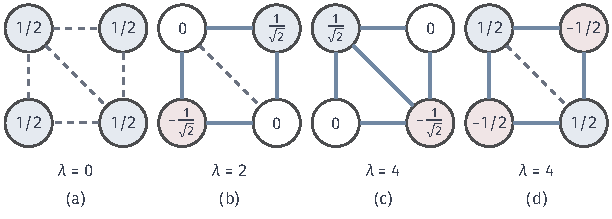
\includegraphics{figures/03-graphs/05-matrices-and-spectra/tikz/laplacian-four-modes.pdf}
  \caption{四点单位权图的四个单位特征向量。圆内为该点的坐标，浅蓝、浅红和白色分别表示正、负和零。两端读数不同的边画成实线，读数相等的边画成虚线。每幅图下的特征值就是沿边变化能量。}
  \label{fig:laplacian-four-modes}
\end{BookInlineFigure}

\subsection{特征值估计}
\label{sec:graph-laplacian-eigenvalue-bounds}

即使暂时没有求出全部特征向量，也能从度的信息估计特征值的范围。此外，在固定顶点集上加边后，各特征值只能不减。

先看上界。对单条边$\{i,j\}$，差的平方可以用两端读数各自的平方控制：
\[
  (x_i-x_j)^2\leq 2x_i^2+2x_j^2.
\]
将每条边的这个不等式乘上边权后求和。顶点$i$的$x_i^2$在它的每条邻边中都出现一次，这些边的权重加起来就是$d_i$。因此$x_i^2$的总系数为$2d_i$，从而
\[
  0\leq \bm x^\top\bm L\bm x
  \leq 2\sum_{i=1}^n d_ix_i^2
  \leq 2d_{\max}\lVert\bm x\rVert_2^2,
\]
其中$d_{\max}=\max_i d_i$。令$\bm x$取各单位特征向量，得到
\begin{equation}
  0\leq\lambda_i\leq 2d_{\max},\qquad i=1,\ldots,n.
  \label{eq:graph-laplacian-spectrum-bound}
\end{equation}
最大度给出了所有特征值的统一上界。

接下来考虑加边的影响。在固定的顶点集上增加一条权重为$a\geq0$的新边$e$，拉普拉斯矩阵从$\bm L$变为
\[
  \bm L'=\bm L+a\bm b_e\bm b_e^\top.
\]
新增项$a\bm b_e\bm b_e^\top$是半正定的，因此对任何向量$\bm x$，新图的二次型$\bm x^\top\bm L'\bm x$至少不小于旧图的$\bm x^\top\bm L\bm x$。

要把这个逐向量的比较转化为逐特征值的比较，需要用到 Courant--Fischer 刻画：第$i$个最小特征值等于"先选$i$维子空间，在子空间中求最大的单位能量，再在所有$i$维子空间中取最小值"。可参考\BookChapterRef{chap:condition-and-spectral-perturbation}{卷二"条件数与谱扰动"章}。

固定任何一个$i$维子空间$U$。旧图中在$U$内达到最大单位能量的向量放进新图，能量只会增加或保持，所以新图在$U$内的最大值不会更小。这对每个$U$都成立。在所有$U$中取最小值时，新图的最小值也不会更小。因此
\begin{equation}
  \lambda_i(\bm L')\geq\lambda_i(\bm L),\qquad i=1,\ldots,n.
  \label{eq:graph-laplacian-edge-monotonicity}
\end{equation}
这个比较使用同一个顶点集上的向量空间。删去一个顶点时，向量空间的维数和度都会改变，不能直接套用这个结论。

用四点图来验证。单位权四点环的谱是$0,2,2,4$（下面会给出环图的谱公式）。加入对角边$13$后变为$0,2,4,4$。观察方向$(1,0,-1,0)^\top$，它在新增边上两端读数不同，加入该边后沿边能量增加，这个方向原来对应特征值$2$，现在上升到$4$。另一方向$(0,1,0,-1)^\top$在新增边上两端相等，不受影响，仍对应$2$。

\subsection{典型图的拉普拉斯谱}
\label{sec:graph-typical-laplacian-spectra}

对几类常见图，可以利用它们的结构直接写出谱。正则图的拉普拉斯谱与邻接谱之间有简单的标量关系。

在简单无权的$d$正则图上，每个顶点的度都为$d$，所以$\bm D=d\bm I$。设$\bm x$是邻接矩阵$\bm A$的特征向量，对应特征值$\alpha$。拉普拉斯作用于$\bm x$时，
\[
  \bm L\bm x=(d\bm I-\bm A)\bm x=d\bm x-\alpha\bm x=(d-\alpha)\bm x.
\]
特征向量保持不变，邻接特征值$\alpha$变成了拉普拉斯特征值$d-\alpha$。如果各点度不同，$\bm D$不是标量矩阵，就不能用这种简单的平移换算。

利用这个关系，可以直接把上一章算出的邻接谱转成拉普拉斯谱。

\begin{theorem}[典型图的拉普拉斯谱]
\label{prop:graph-typical-laplacian-spectra}
\leavevmode
\begin{enumerate}
  \item 完全图$K_n$：$0$（重数$1$），$n$（重数$n-1$）。
  \item 环$C_n$（$n\ge3$）：$\lambda_k=2-2\cos(2\pi k/n)$，$k=0,\ldots,n-1$。
  \item 路径$P_n$（$n\ge2$）：$\lambda_k=2-2\cos(k\pi/n)$，$k=0,\ldots,n-1$。
  \item 星$K_{1,n-1}$（$n\ge2$）：$0$（重数$1$），$1$（重数$n-2$），$n$（重数$1$）。
\end{enumerate}
\end{theorem}

\paragraph{完全图}

对完全图$K_n$，邻接谱为$n-1$（重数$1$）和$-1$（重数$n-1$），度$d=n-1$，拉普拉斯谱为$0$（重数$1$）和$n$（重数$n-1$）。

\paragraph{环}

对环图$C_n$（$n\geq3$），邻接特征值为$2\cos(2\pi k/n)$，度$d=2$，拉普拉斯特征值为
\begin{equation}
  \lambda_k^{(C)}=2-2\cos(2\pi k/n),\qquad k=0,\ldots,n-1.
  \label{eq:graph-cycle-laplacian-spectrum}
\end{equation}
$k$是模态编号，写出的顺序不一定是特征值的升序。取$n=4$得到$0,2,4,2$，排序后为$0,2,2,4$，与四点环未加对角线时的谱一致。

\paragraph{路径}

对路径$P_n$，因为端点只有一个邻居。内部顶点$i$的拉普拉斯输出是$2x_i-x_{i-1}-x_{i+1}$。端点$1$只有右邻点$2$，输出是$x_1-x_2$。

为了统一处理端点和内部顶点，我们在左端外添一个辅助坐标$x_0=x_1$。此时
\[
  2x_1-x_0-x_2=2x_1-x_1-x_2=x_1-x_2,
\]
与端点的真实输出一致。等值的辅助坐标没有引入新的沿边差异。右端同样用$x_{n+1}=x_n$。

接下来找满足$x_{i-1}+x_{i+1}=\lambda x_i$的模式。尝试$x_i=\cos\bigl((i-\tfrac12)\theta\bigr)$，其中$\theta$是相邻读数的相位差。利用三角和差公式可得$x_{i-1}+x_{i+1}=2\cos\theta\cdot x_i$，因此内部顶点上的特征值为$2-2\cos\theta$。

左端的辅助条件自动满足：$\cos(-\theta/2)=\cos(\theta/2)$，余弦的偶性保证了$x_0=x_1$。右端的条件要求
\[
  x_{n+1}-x_n=-2\sin(n\theta)\sin(\theta/2)=0.
\]
取$\theta=k\pi/n$，$k=0,\ldots,n-1$，每个角度给出一个非零向量。$n$个不同的特征值为
\begin{equation}
  \lambda_k^{(P)}=2-2\cos(k\pi/n),\qquad k=0,\ldots,n-1.
  \label{eq:graph-path-laplacian-spectrum}
\end{equation}
其中半格偏移$\tfrac12$对应两端保持相同读数的边界条件，这与邻接矩阵路径公式所用的两端为零条件不同。

\paragraph{星图}

对星图$K_{1,n-1}$（$n\geq2$），设中心读数为零，各叶读数之和也为零。每片叶只与中心相连，输出等于自己的读数减去中心读数，即等于自己。中心读取所有叶的差值之和，由于叶总和为零，输出也为零。这给出维数$n-2$、特征值为$1$的子空间。

剩下两个方向可以取常向量（特征值$0$）和"中心为$n-1$、各叶为$-1$"的向量。后者在每条边上相差$n$，中心的邻居和为$(n-1)\cdot(-1)$，输出为$(n-1)(n-1-(- 1))=n(n-1)$。等等，这里更直接地算：各点的$\bm L$作用下，中心输出$d_{\text{center}}\cdot(n-1)-\sum_{\text{leaves}}(-1)=(n-1)(n-1)+(n-1)=n(n-1)$，而每片叶输出$1\cdot(-1-(n-1))=-n$。因此$\bm L\bm x=n\bm x$，特征值为$n$。四顶点星图的谱为$0,1,1,4$。虽然和四点路径一样有四个顶点三条边，两者的拉普拉斯谱完全不同。

\paragraph{补图}

最后看补图的谱换算。对简单无权图$\mathcal G$，它与补图$\overline{\mathcal G}$的边合在一起构成完全图，且没有重复。因此
\begin{equation}
  \bm L(\overline{\mathcal G})
  =\bm L(K_n)-\bm L(\mathcal G)
  =n\bm I-\bm1\bm1^\top-\bm L(\mathcal G).
  \label{eq:graph-complement-laplacian}
\end{equation}
常向量$\bm1$对两张图都是零方向。沿与常向量正交的原图特征向量$\bm u_i$（$i\geq2$），$\bm1\bm1^\top\bm u_i=\bm0$，因此补图的特征值变成$n-\lambda_i$。如果原图恰好有某个特征值等于$n$，补图在该方向上的特征值为零，对应一个额外的零方向——由定理~\ref{thm:graph-laplacian-components}可知，补图多了一个连通分量。
